\documentclass[11pt,a4paper]{article}

% --------------------------------------------------------
% PACOTES
% --------------------------------------------------------
\usepackage[brazil]{babel}
\usepackage[utf8]{inputenc}
\usepackage[T1]{fontenc}
\usepackage{amsmath}

\usepackage[top=1.5cm, bottom=1.5cm, left=1.8cm, right=1.8cm]{geometry}

% Fonte sem serifa (Computer Modern Sans - já incluída em qualquer instalação TeX,
% sem depender de pacotes de fonte externos como o urw-base35)
\renewcommand{\familydefault}{\sfdefault}

\usepackage{graphicx}
\usepackage{array}
\usepackage{booktabs}
\usepackage{float}
\usepackage{caption}
\usepackage[table]{xcolor}
\usepackage{enumitem}
\setlist{noitemsep, topsep=1pt, leftmargin=1.3em, parsep=0pt}
\usepackage[colorlinks=true, linkcolor=black, citecolor=black, urlcolor=blue]{hyperref}

% Espaçamento mais compacto de \section/\subsection sem depender do pacote
% titlesec (usa só o mecanismo \@startsection do núcleo do LaTeX).
\makeatletter
\renewcommand{\section}{\@startsection{section}{1}{0pt}{7pt}{3pt}{\normalfont\large\bfseries}}
\renewcommand{\subsection}{\@startsection{subsection}{2}{0pt}{5pt}{2pt}{\normalfont\bfseries}}
\makeatother

\setlength{\parindent}{0pt}
\setlength{\parskip}{0.22em}
\captionsetup{font=footnotesize, labelfont=bf, skip=2pt}
\renewcommand{\arraystretch}{0.92}

\newcommand{\code}[1]{\texttt{\footnotesize #1}}

% --------------------------------------------------------
% METADADOS
% --------------------------------------------------------
\title{Modelo Vetorial e BM25 sobre a Coleção Cranfield}
\author{}
\date{}

\begin{document}
\pagestyle{plain}

\begin{center}
{\Large \textbf{Modelo Vetorial e BM25 sobre a Coleção Cranfield}}\\[1pt]
{\normalsize Implementação, Avaliação e Análise de Erros}\\[6pt]
{\normalsize Gustavo Blois, NUSP 13688612}\\
\footnotesize Instituto de Ciências Matemáticas e de Computação, Universidade de São Paulo (ICMC/USP),
\texttt{gustavobloisrr@usp.br}\\
\footnotesize Trabalho Prático 1, SCC0282 Recuperação de Informação, 2º Sem/2026, Prof. Marcelo Manzato
\end{center}
\vspace{2pt}\hrule\vspace{6pt}

% ========================================================
\section{Introdução}
% ========================================================

Sistemas de Recuperação de Informação (RI) ordenam documentos de uma coleção de acordo com sua
relevância estimada para uma consulta. A coleção \textbf{Cranfield} (1400 resumos de artigos de
engenharia aeronáutica, cobrindo aerodinâmica, estruturas, transferência de calor e aeroelasticidade, e
225 consultas com julgamentos de relevância graduados) é um dos primeiros e mais usados
\textit{benchmarks} para avaliar esses sistemas.

Este trabalho implementa, sem bibliotecas de RI que escondam o cálculo do \textit{score}, dois modelos
clássicos, o \textbf{modelo vetorial} (\textit{tf-idf} com similaridade de cosseno) e o
\textbf{modelo probabilístico BM25}, e os avalia com as métricas usuais. O objetivo não é só medir qual
modelo tem a maior média, mas entender \emph{por que} os dois discordam em certas consultas: como o
pré-processamento, o comprimento dos documentos e a forma como cada modelo pondera a repetição de um
termo interagem para produzir rankings diferentes, e, em alguns casos, igualmente ruins.

% ========================================================
\section{Técnicas Utilizadas}
% ========================================================

\subsection{Pré-processamento}
O texto passa por tokenização, normalização para minúsculas, remoção de \textit{stopwords} (lista fixa
de 36 palavras em inglês) e \textit{stemming} (Snowball para o inglês, pacote opam \code{stem}). As
quatro configurações do item 1 ligam/desligam essas duas etapas independentemente: \code{raw},
\code{stopwords}, \code{stemming}, \code{stopwords+stemming}.

\subsection{Índice invertido}
O índice invertido é uma \textbf{hashtable de hashtables}: termo~$\to$~(id do documento~$\to$~tf).
Verificar se um termo ocorre em um documento e obter sua frequência são, portanto, duas buscas em
hashtable encadeadas, cada uma $O(1)$ esperado, em vez de uma busca linear em postings ou um acesso a
uma matriz densa termo-documento.

O custo fica na \emph{construção}: montar o índice exige um passe por todos os tokens de todos os
documentos, $O(D \cdot \bar{W}) = O(\sum_d |d|)$, com $D=1400$ documentos e $\bar{W}\approx 99{,}85$ o
comprimento médio de documento (\code{avgdl}). Cada inserção é $O(1)$ amortizado, então o total é linear
no corpus. O mesmo custo aparece ao montar as estatísticas globais (idf de cada termo, norma de cada
documento): outro passe $O(\sum_d |d|)$, feito uma única vez e reaproveitado pelas 225 consultas. Como o
BM25 e o vetorial só percorrem as \textit{posting lists} dos termos da consulta, o custo de pontuar uma
consulta é $O\!\left(\sum_{t\in q} df(t)\right)$: proporcional a quão comuns são seus termos, não ao
tamanho da coleção. O preço desse ganho por consulta é pagar, uma única vez, essa construção mais cara.

\subsection{Modelo vetorial}
Documentos e consultas são vetores no espaço dos termos do vocabulário, com peso
$w(t,x) = (1+\ln tf(t,x)) \cdot \ln(N/df(t))$ (tf logarítmico, idf logarítmico; sem normalização de
documento na fórmula do peso porque o cosseno já normaliza):
$\cos(q,d) = \dfrac{\sum_t w(t,q)\,w(t,d)}{\lVert q\rVert\, \lVert d\rVert}$ mede o ângulo entre os
vetores, isto é, se consulta e documento enfatizam os mesmos termos proporcionalmente, independente do
tamanho absoluto de cada um.

\subsection{BM25}
Implementado termo a termo (\code{lib/model.ml}), percorrendo a \textit{posting list} de cada termo da
consulta:
\[
\text{score}(d,q) = \sum_{t \in q} idf(t) \cdot \frac{tf(t,d)\,(k_1+1)}{tf(t,d) + k_1\left(1-b+b\,\dfrac{|d|}{avgdl}\right)},
\quad idf(t) = \ln\!\left(1 + \frac{N - df(t) + 0{,}5}{df(t)+0{,}5}\right)
\]
$k_1$ controla a saturação da frequência de termo; $b$ controla a normalização por tamanho do documento
(em $b{=}0$ o termo entre parênteses vale sempre 1; em $b{=}1$ ele é $|d|/avgdl$). Diferente do
vetorial, o BM25 não normaliza pelo tamanho da consulta e soma contribuições independentes por termo.

\subsection{Métricas}
Precision@10, Recall@10, F1@10, AP@\emph{all} (média = MAP), AP@10, \textit{Reciprocal Rank} (média =
MRR) e NDCG@10 (ganho $g=5-\text{grau}$, desconto $\log_2$), calculadas por consulta e agregadas por
média. Nas métricas binárias, relevante = grau~$\geq 1$; grau~$-1$ e não julgados contam como não
relevantes.

\subsection{Ferramentas auxiliares}
Todo o pipeline foi implementado em OCaml sem biblioteca de RI; só o \textit{stemming} usa o pacote opam
\code{stem}. Os gráficos deste relatório foram gerados com \textbf{gnuplot}, a partir de \textit{scripts}
\code{.gp} escritos pelo próprio programa (\code{recinf plot}), reprodutíveis junto com os experimentos.

% ========================================================
\section{Avaliação}
% ========================================================

\textbf{Dataset:} Cranfield, obtida em
\href{https://ir.dcs.gla.ac.uk/resources/test_collections/cran/}{University of Glasgow, Cranfield Collection}
(1400 documentos, 225 consultas, qrels \code{consulta doc grau}). Os ids do arquivo de consultas não
coincidem com a numeração dos qrels (que numera as consultas de 1 a 225 pela posição); o programa usa
essa posição, mostrando também o id original quando relevante.

\textbf{Configurações:} 4 pré-processamentos $\times$ (vetorial + BM25 em grade
$k_1\in\{0{,}5;1{,}2;2{,}0\}$ $\times$ $b\in\{0;0{,}75;1\}$) = 40 execuções, cada uma nas 225 consultas.
Resultados por consulta (\code{results/per\_query.csv}) e agregados (\code{results/summary.csv}). Para
comparar vetorial e BM25 em cada configuração, conto quantas consultas cada um vence, quantas empatam e
quantas têm diferença ``clara'' ($|\Delta AP| \geq 0{,}1$) (\code{results/comparison\_summary.csv}).

% ========================================================
\section{Resultados Obtidos e Análise}
% ========================================================

\subsection{Efeito do pré-processamento (Item 1)}

\begin{table}[H]
\centering\footnotesize
\begin{tabular}{lrrrrrrr}
\toprule
Pré-proc. & Modelo & P@10 & R@10 & F1@10 & MAP & MRR & NDCG@10 \\
\midrule
raw                & vetorial & 0,2049 & 0,3361 & 0,2307 & 0,2506 & 0,4742 & 0,3051 \\
raw                & BM25     & 0,2098 & 0,3469 & 0,2367 & 0,2544 & 0,4926 & 0,3182 \\
stopwords          & vetorial & 0,2067 & 0,3396 & 0,2329 & 0,2500 & 0,4728 & 0,3061 \\
stopwords          & BM25     & 0,2124 & 0,3540 & 0,2405 & 0,2559 & 0,4954 & 0,3224 \\
stemming           & vetorial & 0,2164 & 0,3738 & 0,2476 & 0,2722 & 0,4851 & 0,3271 \\
stemming           & BM25     & 0,2169 & 0,3702 & 0,2472 & 0,2834 & 0,5305 & 0,3446 \\
stopwords+stemming & vetorial & \textbf{0,2173} & \textbf{0,3741} & \textbf{0,2483} & \textbf{0,2722} & 0,4849 & 0,3279 \\
stopwords+stemming & BM25     & \textbf{0,2182} & 0,3730 & \textbf{0,2489} & \textbf{0,2861} & 0,5297 & \textbf{0,3481} \\
\bottomrule
\end{tabular}
\vspace{-2pt}
\caption{Métricas médias por pré-processamento (BM25 com $k_1{=}1{,}2,\,b{=}0{,}75$).}
\end{table}

\vspace{-6pt}
\begin{figure}[H]
\centering
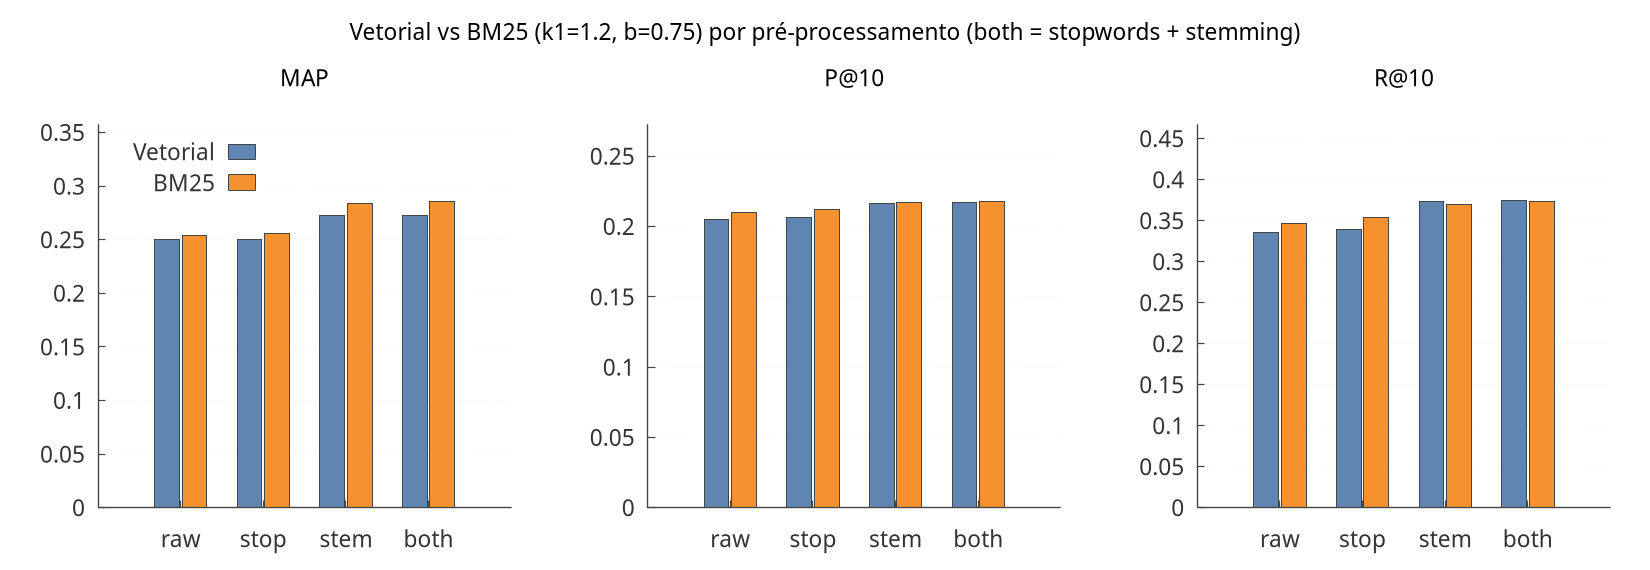
\includegraphics[width=0.9\textwidth]{results/plots/metrics_by_preprocessing.png}
\vspace{-4pt}
\caption{MAP, P@10 e R@10 por pré-processamento, vetorial vs.\ BM25.}
\end{figure}
\vspace{-8pt}

O ganho relevante vem do \textit{stemming}: as seis métricas melhoram com ele, nos dois modelos, então a
conclusão não depende de olhar só uma. Uso o MAP para resumir os números por ser a única que considera o
\textit{ranking} inteiro, não só os 10 primeiros: MAP vetorial $0{,}2506\to0{,}2722$; BM25
$0{,}2544\to0{,}2861$. O \textit{stemming} une variações morfológicas de um mesmo conceito (p.ex.\
\textit{ablate}/\textit{ablating}/\textit{ablation} $\to$ \code{ablat}) que, sem ele, nunca casariam
entre consulta e documento. Ele também erra no sentido oposto, separando palavras que deveriam ficar
juntas: \textit{rarefaction} (consulta 52) vira \code{rarefact}, mas \textit{rarefied} (em documentos
sobre escoamento hipersônico rarefeito) vira \code{rarefi}: a mesma ideia, duas formas, dois stems
diferentes (outro caso assim, verificado termo a termo, na Seção~\ref{sec:erros}).

A remoção de \textit{stopwords} isoladamente quase não muda o MAP ($0{,}2506\to0{,}2500$ no vetorial),
porque essas palavras já recebem idf baixo nos dois modelos: removê-las tira ruído que já pesava pouco.
Combinar as duas técnicas não soma os ganhos (MAP igual ao de \textit{stemming} isolado): a maior parte
do efeito já vem dele.

\subsection{Vetorial vs.\ BM25 (Item 5)}

\begin{table}[H]
\centering\footnotesize
\begin{tabular}{lrrrrrr}
\toprule
Métrica & vetorial & BM25 & $\Delta$ & venc. BM25 & venc. vetor. & empates \\
\midrule
MAP      & 0,2722 & 0,2861 & +0,0139 & 125 & 91 & 9   \\
MAP@10   & 0,2153 & 0,2284 & +0,0131 & 106 & 67 & 52  \\
P@10     & 0,2173 & 0,2182 & +0,0009 & 51  & 43 & 131 \\
R@10     & 0,3741 & 0,3730 & -0,0012 & 51  & 43 & 131 \\
MRR      & 0,4849 & 0,5297 & +0,0448 & 86  & 54 & 85  \\
NDCG@10  & 0,3279 & 0,3481 & +0,0202 & 111 & 67 & 47  \\
\bottomrule
\end{tabular}
\vspace{-2pt}
\caption{Vetorial vs.\ BM25 ($k_1{=}1{,}2$, $b{=}0{,}75$, stopwords+stemming), 225 consultas.}
\end{table}

O BM25 vence mais consultas do que perde em todas as métricas, mas a margem varia: ganho relativo de
$+9{,}2\%$ em MRR contra $+0{,}4\%$ em P@10 e empate técnico em R@10 (131/225). Isso combina com a
definição de cada métrica: o MRR depende só da posição do primeiro relevante (seu inverso), então um
ganho grande nele indica que o BM25 acha o primeiro documento útil mais cedo. P@10/R@10 só contam
quantos relevantes entram no corte de 10, sem ligar para a ordem entre eles; o BM25 ganhar pouco aí
mostra que essa vantagem reordena o \textit{ranking}, mas não coloca \emph{mais} relevantes dentro do
corte (o MAP, que olha o \textit{ranking} inteiro, também capta essa reordenação).

\subsection{Análise por consulta (Item 6)}
\label{sec:item6}

\begin{figure}[H]
\centering
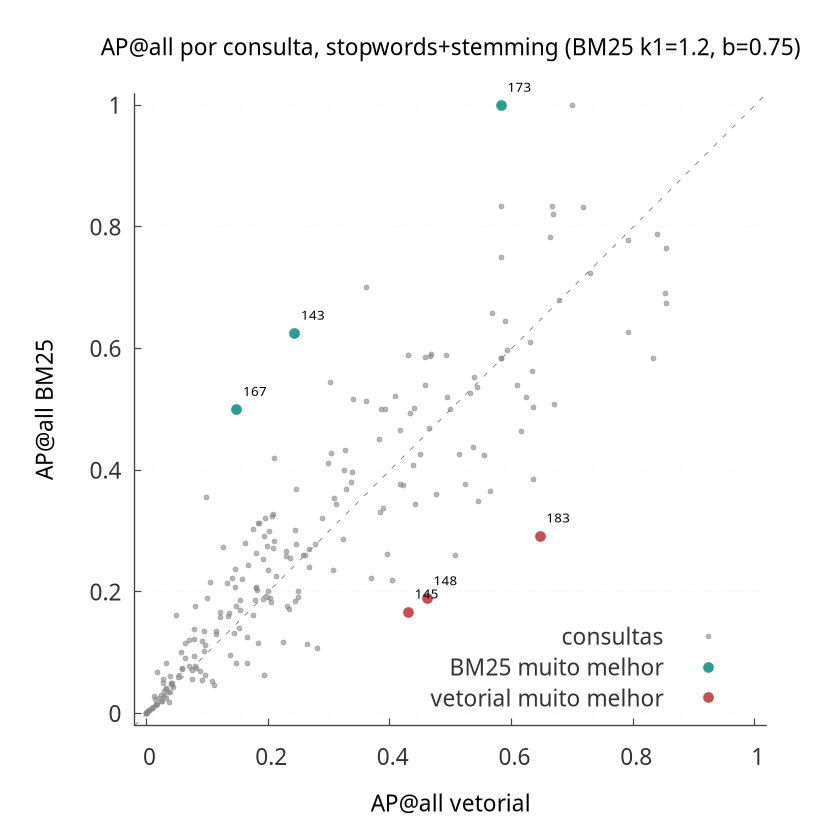
\includegraphics[width=0.6\textwidth]{results/plots/scatter_ap.png}
\vspace{-4pt}
\caption{AP@\emph{all} por consulta, vetorial vs.\ BM25; consultas do item 6 destacadas.}
\end{figure}
\vspace{-6pt}

\begin{table}[H]
\centering\footnotesize
\begin{tabular}{clp{7.3cm}r}
\toprule
Q (.I) & Modelo & Top-5 (\textsuperscript{g} = grau de relevância, 1 = melhor) & AP \\
\midrule
\multicolumn{4}{l}{\textit{BM25 muito melhor}} \\
173 (264) & vetorial & 532, 367\textsuperscript{1}, 451\textsuperscript{1}, 917, 29        & 0,583 \\
173 (264) & BM25     & 367\textsuperscript{1}, 451\textsuperscript{1}, 532, 767, 917        & 1,000 \\
143 (213) & vetorial & 1068, 930, 1043\textsuperscript{1}, 828, 953                          & 0,244 \\
143 (213) & BM25     & 1043\textsuperscript{1}, 1068, 930, 1134, 828                         & 0,625 \\
\midrule
\multicolumn{4}{l}{\textit{Vetorial muito melhor}} \\
183 (277) & vetorial & 1243\textsuperscript{4}, 804\textsuperscript{4}, 1247\textsuperscript{4}, 808\textsuperscript{1}, 811\textsuperscript{3} & 0,647 \\
183 (277) & BM25     & 893, 811\textsuperscript{3}, 1226, 804\textsuperscript{4}, 808\textsuperscript{1} & 0,292 \\
148 (218) & vetorial & 1048\textsuperscript{2}, 1050\textsuperscript{2}, 956, 1126, 761       & 0,462 \\
148 (218) & BM25     & 956, 1126, 1048\textsuperscript{2}, 1050\textsuperscript{2}, 928       & 0,189 \\
\midrule
\multicolumn{4}{l}{\textit{Ambos fracos}} \\
13 (26)   & vetorial & 496, 903, 643, 313, 520                                                & 0,000 \\
13 (26)   & BM25     & 496, 903, 520, 313, 38                                                 & 0,000 \\
44 (79)   & vetorial & 1190, 862, 385, 1148, 236                                              & 0,000 \\
44 (79)   & BM25     & 103, 108, 1190, 1199, 1072                                             & 0,000 \\
\bottomrule
\end{tabular}
\vspace{-2pt}
\caption{Top-5 documentos das seis consultas do item 6 (sem sobrescrito = não relevante).}
\end{table}

\textbf{BM25 muito melhor.} Em Q173 (2 relevantes), AP $0{,}583\to\mathbf{1{,}000}$. O não relevante mais
bem colocado no vetorial (532, sobre estabilidade de mísseis) repete o termo raro \code{lyapunov} 3
vezes contra 2 no relevante 367, e por ser mais curto ($|d|{=}25{,}2$ vs.\ $35{,}4$) tem norma menor: sua
similaridade ($0{,}432$) supera a do 367 ($0{,}299$), mesmo o 367 casando com \emph{mais} termos da
consulta (\code{linear}, \code{differenti}, \code{equat}, além de \code{lyapunov}/\code{stabil}). No
BM25, a saturação de \textit{tf} reduz a vantagem da repetição extra no 532 (contribuição $11{,}64$ vs.\
$9{,}68$ no 367), enquanto o 367 soma as contribuições dos termos extras ($+8{,}33$), superando o 532
($23{,}09$ vs.\ $18{,}07$). O cosseno recompensa foco estreito em um termo raro; o BM25 recompensa cobrir
mais termos, porque cada um soma um valor próprio sem ser diluído pela norma do documento inteiro. Q143
segue o padrão: o único relevante no top-5 (1043) sobe da 3\textsuperscript{a} posição no vetorial para
a 1\textsuperscript{a} no BM25.

\textbf{Vetorial muito melhor.} Em Q183 (13 relevantes), AP $\mathbf{0{,}647}\to0{,}292$: o vetorial
acerta os 5 primeiros com relevantes de vários graus. No BM25, o documento 893 (sobre calibração de
tubos de Pitot, não relevante) fica em 1\textsuperscript{o} (score $15{,}29$) sem compartilhar
\emph{nenhum} termo temático da consulta (\code{sonic}, \code{boom}, \code{strength}); ele casa só com
\code{what}, \code{factor}, \code{have}, \code{been}. A lista de \textit{stopwords} usada não inclui
essas palavras interrogativas/auxiliares, e nesta coleção elas são raras o bastante (\code{what}
aparece em só 16 dos 1400 documentos) para receber um idf alto ($4{,}44$) sem carregar sinal sobre o
assunto. Como o BM25 soma contribuições termo a termo, essas quatro palavras genéricas bastam para
superar os documentos realmente relevantes; o vetorial sofre menos porque o mesmo produto interno é
dividido pela norma do documento inteiro, que aqui inclui muitos outros termos irrelevantes ao
\code{score}. Q148 é parecida: os dois relevantes do top-5 (1048, 1050) vão de
1\textsuperscript{o}/2\textsuperscript{o} no vetorial para 3\textsuperscript{o}/4\textsuperscript{o} no
BM25.

\textbf{Ambos fracos.} Em Q13 (4 relevantes) e Q44 (3 relevantes), AP $=0$ nos dois modelos: nenhum
relevante aparece entre os 30 primeiros. Q13 é o caso mais revelador: o documento mais bem colocado por
ambos (496, título quase idêntico ao da consulta: ``a theory of transonic aileron buzz\dots'') está
marcado como \textbf{não relevante} (grau $-1$) nos qrels; os 4 relevantes de fato (64, 265, 65, 311)
tratam do mesmo fenômeno (interação onda de choque/camada limite) com vocabulário totalmente diferente
(``shock wave'', ``boundary layer'', ``vorticity''), sem usar \code{aileron} ou \code{buzz}. O problema
não é erro de cálculo, é a suposição de que casamento lexical implica relevância: o julgamento do
Cranfield reflete uma noção de assunto mais profunda do que a sobreposição de palavras. Q44 é análoga: a
consulta menciona a teoria ``chapman-enskog'', termo raro ausente dos 3 documentos relevantes.

\subsection{Parâmetros do BM25 (Item 7)}

\begin{table}[H]
\centering\footnotesize
\begin{tabular}{rrrrrrr}
\toprule
& \multicolumn{3}{c}{MAP} & \multicolumn{3}{c}{NDCG@10} \\
$k_1 \backslash b$ & 0 & 0,75 & 1 & 0 & 0,75 & 1\\
\midrule
0,5 & 0,2434 & 0,2689 & 0,2707 & 0,2980 & 0,3317 & 0,3315 \\
1,2 & 0,2508 & \textbf{0,2861} & 0,2851 & 0,3067 & 0,3481 & 0,3452 \\
2,0 & 0,2508 & \textbf{0,2917} & 0,2886 & 0,3100 & \textbf{0,3538} & 0,3510 \\
\bottomrule
\end{tabular}
\vspace{-2pt}
\caption{Grade de parâmetros do BM25 (stopwords+stemming), 225 consultas.}
\end{table}

\vspace{-6pt}
\begin{figure}[H]
\centering
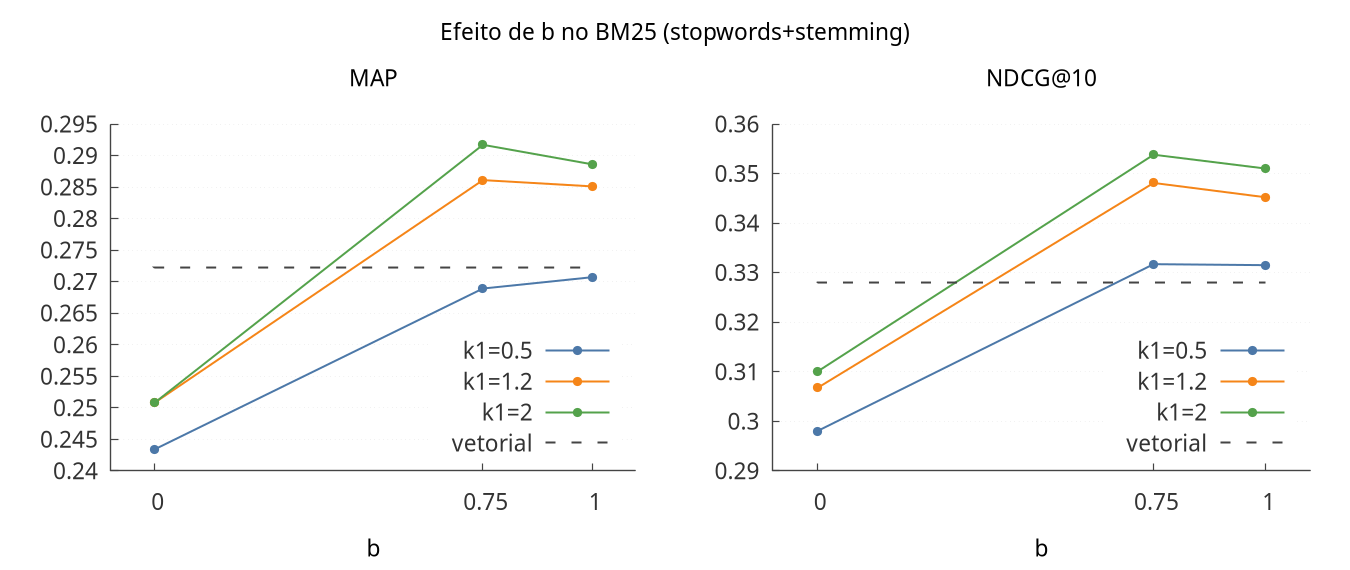
\includegraphics[width=0.8\textwidth]{results/plots/bm25_b_effect.png}
\vspace{-4pt}
\caption{Efeito de $b$ no BM25 por $k_1$; tracejado = vetorial.}
\end{figure}
\vspace{-8pt}

$b$ tem efeito muito maior que $k_1$: $b{=}0\to0{,}75$ ganha até $0{,}04$ de MAP em qualquer $k_1$,
enquanto variar $k_1$ com $b$ fixo move o MAP em no máximo $0{,}007$. Nesta coleção, normalizar pelo
tamanho do documento importa mais que ajustar a saturação de \textit{tf}: os documentos variam bastante
em tamanho, e sem normalização ($b{=}0$) os longos acumulam \textit{tf} bruto só por serem longos.
$b{=}1$ não ajuda mais que $b{=}0{,}75$: a normalização completa penaliza demais alguns relevantes que
são naturalmente mais longos que a média.

\textbf{Consulta sensível a $b$: Q52.} AP $0{,}207$ ($b{=}0$) $\to$ $\mathbf{0{,}850}$ ($b{=}1$),
$k_1{=}1{,}2$. Com $b{=}0$, o documento 798 (não relevante, $|d|{=}382$, quase $4\times$ a média) fica em
1\textsuperscript{o}, na frente do relevante 326 (grau 4, $|d|{=}32$, bem mais curto que a média): sem
normalização, o documento longo acumula mais ocorrências brutas só por ter mais texto. Com $b{=}1$, o
798 é penalizado proporcionalmente ao tamanho e o 326 assume a liderança (P@10 $0{,}20\to0{,}40$, os 4
relevantes entram no \textit{ranking}): exatamente o efeito que $b$ deveria produzir.

\subsection{Modificação de consultas (Item 8)}
\label{sec:item8}

Cinco consultas foram escolhidas e reformuladas manualmente (ferramenta de apoio descrita na
Seção~\ref{sec:ia}); resultados completos em \code{results/modifications.csv}.

\begin{table}[H]
\centering\footnotesize
\begin{tabular}{p{0.55cm}p{5.0cm}rr}
\toprule
Q (.I) & mudança & AP vetor & AP BM25 \\
\midrule
14 (27)  & removeu ``papers on''                                       & 0,076 $\to$ 0,667 & 0,071 $\to$ 0,700 \\
35 (61)  & sinônimo ``acoustic''$\to$``sound'' + removeu \textit{boilerplate} & 0,025 $\to$ 0,394 & 0,021 $\to$ 0,178 \\
17 (32)  & reformulação mais explícita                                 & 0,508 $\to$ 0,506 & 0,260 $\to$ 0,507 \\
6 (10)   & removeu ``theoretical and experimental \dots do we have''   & 0,050 $\to$ 0,075 & 0,160 $\to$ 0,171 \\
22 (40)  & reescrita com o vocabulário do documento relevante          & 0,000 $\to$ \textbf{1,000} & 0,000 $\to$ \textbf{1,000} \\
\bottomrule
\end{tabular}
\vspace{-2pt}
\caption{As cinco modificações, AP@\emph{all} antes $\to$ depois.}
\end{table}

Q14 e Q35 mostram o mesmo padrão: as consultas originais têm frases de preenchimento (``papers on'',
``are there any \dots dealing with'') que competem por peso contra os termos de conteúdo; ao removê-las,
o \textit{score} relativo do que importa sobe e os relevantes emergem nos dois modelos. Q17 reforça o
achado da Seção~\ref{sec:item6}: o BM25 responde melhor a uma reformulação que acrescenta termos que
casam com mais relevantes ($0{,}260\to0{,}507$), enquanto o cosseno, sensível à norma do documento,
quase não se altera ($0{,}508\to0{,}506$).

Q22 é o caso mais extremo, continuação direta da Seção~\ref{sec:erros}: como o documento relevante 68
não compartilha \emph{nenhum} \textit{stem} com a consulta original, a reformulação foi construída
lendo o resumo do documento 68 e reescrevendo a consulta com esse vocabulário (\textit{air},
\textit{helium}, \textit{simulation}, \textit{viscous}, \textit{hypersonic}). O resultado (AP $0\to1$
nos dois modelos) confirma o diagnóstico, mas com uma ressalva: não é uma troca por sinônimos da
consulta original, é uma reescrita apoiada no texto do documento-alvo, uma forma de
\textit{expansão de consulta com oráculo} (escrita sabendo qual é o documento certo), mais forte do que
uma reformulação real feita sem conhecer a resposta.

\subsection{Análise de erros (Item 9)}
\label{sec:erros}

O comando \code{recinf errors} lista, por consulta, os documentos não relevantes nas 5 primeiras
posições (falsos positivos) e os relevantes fora do Top-10, inclusive nunca recuperados (falsos
negativos); lista completa em \code{results/error\_analysis.csv}. Dela, dois falsos positivos e um falso
negativo entre os mais claros de explicar:

\begin{enumerate}
\item \textbf{Falso positivo: Q13, doc.\ 496} (1\textsuperscript{o} nos dois modelos, grau $-1$), já
discutido na Seção~\ref{sec:item6}: título quase idêntico à consulta, mas explicitamente não relevante;
os de fato relevantes usam vocabulário totalmente diferente para o mesmo fenômeno. O doc.\ 265, por
exemplo, descreve exatamente o \textit{aileron buzz} sem usar essas palavras: \textit{aileron} vira
``control surface'', \textit{buzz} vira ``instabilities''/``oscillatory behaviour'', e o
\textit{mechanism} perguntado na consulta é descrito como ``interaction between shock waves and
boundary layer''.
\item \textbf{Falso positivo: Q3, doc.\ 485} (``linear heat flow in a composite slab'',
1\textsuperscript{o}, cosseno $0{,}46$, BM25 $21{,}1$): a consulta é majoritariamente frase de
preenchimento; só \code{composit} ($df{=}23$) e \code{slab} ($df{=}14$) carregam sinal, ambos raros, e
bastam para o documento liderar nos dois modelos.
\item \textbf{Falso negativo: Q22, doc.\ 68} (único relevante, grau 1, \textbf{nunca recuperado}, score
$=0$): nenhum \textit{stem} da consulta ocorre no documento. Ele contém \textit{viscous}; a consulta usa
\textit{viscosity}. Deveriam casar, mas o \textit{stemmer} reduz \textit{viscosity} a \code{viscos} e
mantém \textit{viscous} como \code{viscous}: stems diferentes para a mesma família, fechando a única
ponte lexical possível. Nenhum ajuste de $k_1$/$b$ resolve isso, pois o documento nunca entra na lista
de candidatos: é falha de vocabulário, não de \textit{ranking} (ver Seção~\ref{sec:item8}, Q22).
\end{enumerate}

% ========================================================
\section{Considerações Finais}
% ========================================================

O BM25 ganha mais consultas do que perde em todas as métricas, mas a vantagem está concentrada em achar
o primeiro relevante mais cedo (MRR, MAP), não em encaixar mais relevantes num corte fixo de 10
posições (onde P@10/R@10 empatam). Um critério prático de escolha: se a aplicação valoriza um bom
resultado rápido, o MRR mais alto do BM25 pesa a favor dele; se depende de reunir vários relevantes numa
janela fixa, os dois empatam nesta coleção, e a escolha recai em outros critérios (por exemplo,
simplicidade de implementação).

O \textit{stemming} é o ganho de pré-processamento mais importante, mas erra nos dois sentidos (junta
demais em alguns casos, separa demais em outros, como \textit{viscous}/\textit{viscosity}). A lista fixa
de \textit{stopwords}, por não incluir palavras interrogativas/auxiliares, causou diretamente um falso
positivo de alto impacto (Q183); ampliá-la é uma melhoria barata sugerida pelos próprios dados. $b$
importa mais que $k_1$ nesta coleção, coerente com a grande variação de tamanho dos documentos. Por fim,
parte dos casos ruins não é falha de modelo: são consultas cujos relevantes foram julgados por um
critério de assunto mais profundo do que a sobreposição lexical que qualquer um dos dois modelos, ou o
próprio \textit{stemmer}, consegue captar.

% ========================================================
\section{Uso de Ferramentas de IA}
\label{sec:ia}
% ========================================================

Uma ferramenta de IA (Claude Code) foi usada de forma recorrente ao longo do desenvolvimento, como
assistente de programação e de análise: na escrita e depuração de código OCaml, na exploração dos
resultados dos experimentos (por exemplo, checar hipóteses termo a termo com \code{recinf explain}, ou
montar ferramentas auxiliares para navegar pelos dados na escolha de consultas para os itens 6, 8 e 9) e
na organização e redação deste relatório a partir desses resultados. As decisões de modelagem (fórmulas
do vetorial e do BM25, configurações de pré-processamento e de parâmetros avaliadas) e a interpretação
de cada resultado são do autor, que acompanhou e validou cada etapa.

\end{document}
